\section{Project Theory}
In the papers, \citet{Sarasvathy2003203} and \citet{sarasvathy2001causation}, Sarasvathy discusses causation, effectuation the link to near decomposability.
The logic of causation is defining the market, segmenting the customers, targeting the customers and positioning in the market all to reach the customer. 
That is given a particular goal I want to achieve, what ought I to do and what particular path should I take.
Inversely, effectuation is rather looking at the means available and determining what could be done.
Effectuation also assumes that the future is controllable such that we can reduce the need to predict uncertain future events.
The difference between causation and effectuation can be visualised in \cref{fig:causation_effectuation}.
Saravathy's effectuation model was primarily targeted towards the suicide quadrant where the markets and products are new and predictability is low.

\begin{figure}
	\centering
	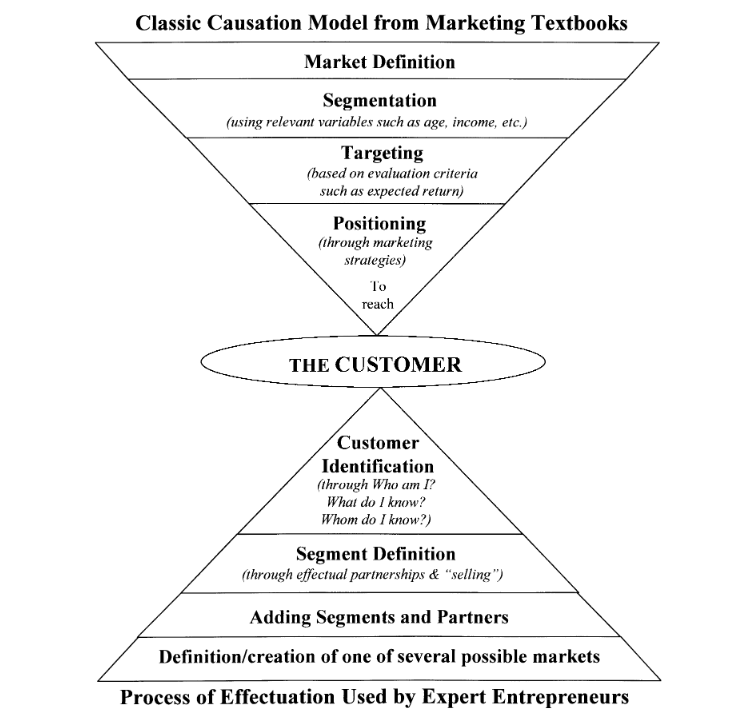
\includegraphics[scale=0.3]{causation_effectuation_pyramid}
	\caption{Effectual contrasting causation from \citet{Sarasvathy2003203}}
	\label{fig:causation_effectuation}
\end{figure}

Causation in relation to this project is the fact that the goal was approached first, and as a result of the goal the rest were examined. 
Effectuation could, however, also be argued for in the sense that the means of the group were examined as a result of that different ideas were examined.
                                                                                                              
In near-decomposable systems the behaviour of components are approximately independent of other components and this creates the effect that systems that are near-decomposable have a higher chance of succeeding in the sense that even if one component in the system fails the entire system will not fail.
We do not believe that our business is near-decomposable, because if it fails gain a market it is necessary to pivot onto a different idea or a different market \citep[pg. 149-178]{ries2011lean}.
But in the case that our customers go bankrupt the company is not severely affected outside of the loss of the subscription license fee. 
In addition, a lot of webshops exists so it should be easy to find other webshops to pay a subscription fee.


\citet{doi:10.1108/S1876-0228(2012)0000009015} challenges the idea of effectuation only being useful in the suicide quadrant and instead that it can be used in other combinations as well.
Kraaijenbrink states that causation and effectuation should be seen as two extremes and it is more beneficial to look at the dimension values that define these models.
As of such the dimensions of these models can be chosen to one's needs, and thus creating a model depending on the market and product.
The dimensions can be seen in \cref{fig:kraaijenbrink}.

The characteristics of our entrepreneurial behaviour are as such:
\begin{description}
	\item[Means-driven vs. Ends-Driven] Means-driven as we have knowledge and experience with recommender systems and try to make a business based on these means.
	\item[Control vs. Prediction] Arguably we have some predictability. That is, we foresee that the e-commerce genre is steadily increasing, and for that reason we believe there is going to be a high demand for high quality recommender systems. The predictability of the business model means it lies outside of the suicide quadrant.
	When it comes to control we cannot pinpoint any specific aspects we can control, one way to control is if we partner with some stakeholder that can affect/control the future in some way, since a lot of the future is affected by human actions/behaviour.
	\item[Affordable loss vs. Expected returns] It is affordable loss since development time is primarily invested for such a business, there is not really any expensive equipment etc. that should be bought. One example of a loss could be if some high tech server is invested in, but for the MVP it is not necessary.
	\item[New products and markets vs. existing products and markets] The product could be either existing or new, in the sense that it could be rationalised as either because the idea of a recommender system is not new but the product itself is new. 
	It is a new market because recommender systems delivered by a third party is not common in Denmark. Something similar exists for a company such as the Hut Group, which is a company that owns over 100 webshops, where they have a centralised backend including recommender systems. That is a company that owns a large amount webshops though, and is not really the market we are targeting, as we are instead targeting webshops where they lack experience or resources to develop a recommender system themselves.
	\item[Cooperation vs. Competition] Cooperation is in focus, as it of utmost importance to gain confidence with the webshops we deliver recommender systems to. We both benefit from the increased sales the recommender system will give.
	\item[Cyclical vs. Linear] Cyclical, we do not indulge in a linear process. That is, we believe the consider-do-adjust paradigm is beneficial, and also follow it since we want to utilise the Lean Startup Build-Measure-Learn loop \citep[pg. 75]{ries2011lean}.
\end{description}

\begin{figure}[!htb]
	\centering
	\includegraphics[scale=0.4]{kraaijenbrink}
	\caption{Human action and entrepreneurial behaviour from \citet{doi:10.1108/S1876-0228(2012)0000009015}}
	\label{fig:kraaijenbrink}
\end{figure}

%Discuss your project theoretically using at least two papers from the syllabus
%
%    Is your choice of paradigm theoretically or empirically justifiable? In what way?
%    Relate your project to concepts from syllabus papers; e.g. effectuation/causation principles✓ , predictability,✓  problem spaces (e.g. suicide quadrant),✓  marketing, lean development, or software development practices.

 